% Figure 1: how the paper reads a prompt, and what sets a description's ESS.
% Compile: latexmk -cd -pdf -interaction=nonstopmode -halt-on-error docs/paper/figs/overview.tex
% ESS values in (b) are copied from ess_curve_sq.csv (d = 16, a0 = 10, n = 0): 15.6, 117, 13.5. Prior shapes are sketches.
%
% Style: the Editorial Neutral system ($visualization-design DESIGN.md), its SVG
% binding translated to TikZ at 0.5 pt per px (16 px node text = 8 pt).
% Color roles: green = the description and its prior, blue = examples,
% pink = the branch where the description is irrelevant. Everything else is gray.
\documentclass[border=0pt]{standalone}
\usepackage[sfdefault]{inter}
\usepackage[T1]{fontenc}
\usepackage[italic]{mathastext}
\usepackage{tikz}
\usetikzlibrary{positioning, calc, decorations.pathreplacing}

\definecolor{ink}{HTML}{171717}
\definecolor{inkmuted}{HTML}{5A5A5A}
\definecolor{inksubtle}{HTML}{8A8A8A}
\definecolor{axis}{HTML}{A8A8A8}
\definecolor{grid}{HTML}{ECECEC}
\definecolor{gray}{HTML}{F5F5F5}
\definecolor{graystroke}{HTML}{B3B3B3}
\definecolor{green}{HTML}{EDF3E8}
\definecolor{greenstroke}{HTML}{8A9F7A}
\definecolor{pink}{HTML}{F5E7EC}
\definecolor{pinkstroke}{HTML}{BD7C8F}
\definecolor{blue}{HTML}{E8F0F9}
\definecolor{bluestroke}{HTML}{7F9FC4}

\tikzset{
  vd/.style={font=\footnotesize, text=ink, line width=0.65pt},
  node/.style={rounded corners=3.5pt, line width=0.65pt, minimum height=6mm,
    minimum width=10mm, inner sep=2pt, text=ink},
  box-gray/.style={node, fill=gray, draw=graystroke},
  box-green/.style={node, fill=green, draw=greenstroke},
  box-blue/.style={node, fill=blue, draw=bluestroke},
  brace/.style={decorate, decoration={brace, amplitude=3pt, raise=1.5mm}, draw=axis, line width=0.6pt},
  lbl/.style={font=\scriptsize, text=inkmuted, align=center},
  header/.style={font=\scriptsize, text=inkmuted, anchor=west, inner sep=0pt},
  panel/.style={font=\footnotesize, text=ink, anchor=west, inner sep=0pt},
  note/.style={font=\scriptsize, anchor=west, align=left},
}

% Inter's Type 1 hyphen carries wide side bearings at small sizes; tighten it.
\newcommand{\hy}{\kern-0.09em-\kern-0.09em}

% One example = one tick, in groups of ten. #1 anchor, #2 whole examples, #3 fraction of the last.
\newcommand{\pitch}{0.63mm}
\newcommand{\gap}{0.35mm}
\newcommand{\sq}{0.44mm}
\newcommand{\tick}{2.4mm}
\newcommand{\exbar}[3]{%
  \foreach \i in {1,...,#2} {\fill[bluestroke] ($(#1)+({(\i-1)*\pitch + int((\i-1)/10)*\gap}, -\tick/2)$) rectangle +(\sq, \tick);}
  \fill[bluestroke] ($(#1)+({#2*\pitch + int(#2/10)*\gap}, -\tick/2)$) rectangle +({#3*\sq}, \tick);
}

% A prior sketch on a 30 mm axis (w from -3 to 3); the description states m = 1.2.
% #1 anchor (left end of the axis), #2 the relevant-description component,
% #3 the irrelevant-description component (0 when reliable).
\newcommand{\prior}[3]{%
  \begin{scope}[shift={(#1)}, x=5mm, y=1.15mm]
    \fill[green, domain=-3:3, samples=160, smooth] plot ({\x+3}, {#2 + #3}) -- (6,0) -- (0,0) -- cycle;
    \fill[pink, domain=-3:3, samples=60, smooth] plot ({\x+3}, {#3}) -- (6,0) -- (0,0) -- cycle;
    \draw[axis, dash pattern=on 2pt off 1.5pt, line width=0.6pt, domain=-3:3, samples=60, smooth]
      plot ({\x+3}, {3*exp(-\x*\x/2)});
    \draw[greenstroke, line width=0.65pt, domain=-3:3, samples=160, smooth] plot ({\x+3}, {#2 + #3});
    \def\wrong{#3}\def\none{0}%
    \ifx\wrong\none\else
      \draw[pinkstroke, line width=0.65pt, domain=-3:3, samples=60, smooth] plot ({\x+3}, {#3});
    \fi
    \draw[axis, line width=0.6pt] (0,0) -- (6,0);
    \draw[axis, line width=0.6pt] (4.2,0) -- (4.2,-0.8) node[below, lbl, inner sep=1pt] {$m$};
  \end{scope}
}

% The true task on a prior's axis. #1 anchor (left end of the axis), #2 its position in w (-3 to 3), #3 color.
\newcommand{\truetask}[3]{%
  \begin{scope}[shift={(#1)}, x=5mm, y=1.15mm]
    \fill[#3] ({#2+3}, 0) circle (0.42mm);
  \end{scope}
}

\begin{document}
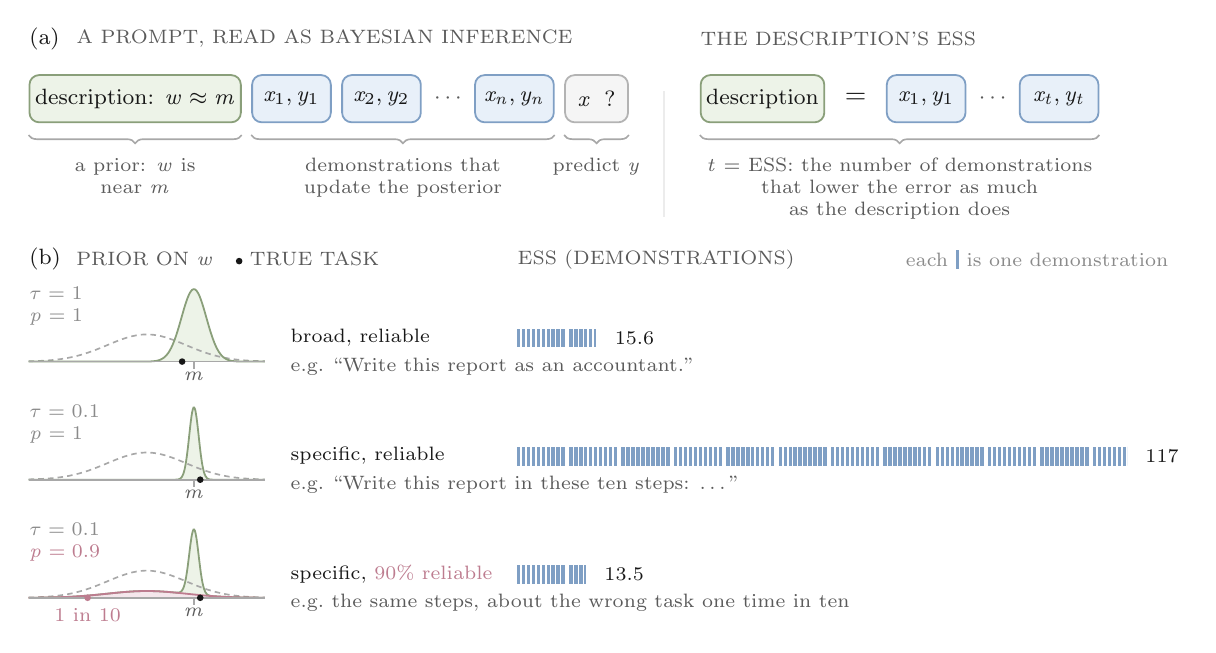
\begin{tikzpicture}[vd]

  % ---------- (a) the prompt as Bayesian inference, and the ESS ----------
  \node[panel, font=\footnotesize] at (0,0) {(a)};
  \node[header] at (6mm,0) {A PROMPT, READ AS BAYESIAN INFERENCE};

  \node[box-green, anchor=north west] (d) at (0,-4.5mm) {description: $w \approx m$};
  \node[box-blue, right=1.2mm of d]  (e1) {$x_1, y_1$};
  \node[box-blue, right=1.2mm of e1] (e2) {$x_2, y_2$};
  \node[right=0.3mm of e2, text=inkmuted] (ed) {$\cdots$};
  \node[box-blue, right=0.3mm of ed] (en) {$x_n, y_n$};
  \node[box-gray, right=1.2mm of en, minimum width=8mm] (q) {$x \;\; ?$};

  \draw[brace] (d.south east) -- node[below=9pt, lbl] {a prior: $w$ is\\near $m$} (d.south west);
  \draw[brace] (en.south east) -- node[below=9pt, lbl] {demonstrations that\\update the posterior} (e1.south west);
  \draw[brace] (q.south east) -- node[below=9pt, lbl] {predict $y$} (q.south west);

  \node[box-green, right=9mm of q] (d2) {description};
  \node[right=1.2mm of d2, font=\normalsize] (eq) {$=$};
  \node[box-blue, right=1.2mm of eq] (k1) {$x_1, y_1$};
  \node[right=0.3mm of k1, text=inkmuted] (kd) {$\cdots$};
  \node[box-blue, right=0.3mm of kd] (kk) {$x_t, y_t$};
  \node[header] at (d2.west |- 0,0) {THE DESCRIPTION'S ESS};
  \draw[brace] (kk.south east) -- node[below=9pt, lbl]
    {$t$ = ESS: the number of demonstrations\\that lower the error as much\\as the description does}
    (d2.south west);
  \draw[grid, line width=0.65pt] ($(q.east)!0.5!(d2.west) + (0,1mm)$) -- ++(0,-16mm);

  % ---------- (b) what sets the worth ----------
  \node[panel, font=\footnotesize] at (0,-28mm) {(b)};
  \node[header] at (6mm,-28mm) {PRIOR ON $w$\quad\tikz[baseline=-0.6mm]\fill[ink] (0,0) circle (0.42mm); TRUE TASK};
  \node[header] at (62mm,-28mm) {ESS (DEMONSTRATIONS)};
  \node[note, text=inksubtle, anchor=east] at (146mm,-28mm)
    {each \tikz[baseline=0.3mm]\fill[bluestroke] (0,0) rectangle (\sq,\tick); is one demonstration};

  \coordinate (r1) at (0,-41mm);
  \coordinate (r2) at (0,-56mm);
  \coordinate (r3) at (0,-71mm);

  % Both reliable priors peak at the same height, so width alone shows specificity. The irrelevant component is
  % drawn small (a quarter of the baseline's height; its true weight is a tenth), so it reads as the rare case.
  \prior{r1}{8*exp(-(\x-1.2)*(\x-1.2)/(2*0.1))}{0}
  \prior{r2}{8*exp(-(\x-1.2)*(\x-1.2)/(2*0.0144))}{0}
  \prior{r3}{7.2*exp(-(\x-1.2)*(\x-1.2)/(2*0.0144))}{0.75*exp(-\x*\x/2)}

  % The true task sits under the description's prior: somewhere inside the broad one, at m under the specific
  % one, and, for the unreliable description, at m nine times in ten and elsewhere one time in ten (pink).
  \truetask{r1}{0.9}{ink}
  \truetask{r2}{1.36}{ink}
  \truetask{r3}{1.36}{ink}
  \truetask{r3}{-1.5}{pinkstroke}
  \node[lbl, text=pinkstroke, inner sep=1pt, anchor=north] at ($(r3)+(7.5mm,-0.9mm)$) {1 in 10};

  % Each row: the prior with its two parameters, the kind of description, and one such instruction in words.
  % The instructions are illustrations only (the ESS values are the Gaussian model's).
  \node[note, text=inksubtle, anchor=north west, inner sep=0pt] at ($(r1)+(0,9.6mm)$) {$\tau = 1$\\$p = 1$};
  \node[note, text=inksubtle, anchor=north west, inner sep=0pt] at ($(r2)+(0,9.6mm)$) {$\tau = 0.1$\\$p = 1$};
  \node[note, text=inksubtle, anchor=north west, inner sep=0pt] at ($(r3)+(0,9.6mm)$) {$\tau = 0.1$\\\textcolor{pinkstroke}{$p = 0.9$}};

  \node[note] at ($(r1)+(32mm,3mm)$) {broad, reliable};
  \node[note] at ($(r2)+(32mm,3mm)$) {specific, reliable};
  \node[note] at ($(r3)+(32mm,3mm)$) {specific, \textcolor{pinkstroke}{90\% reliable}};

  \node[note, text=inkmuted] at ($(r1)+(32mm,-0.6mm)$) {e.g.\ ``Write this report as an accountant.''};
  \node[note, text=inkmuted] at ($(r2)+(32mm,-0.6mm)$) {e.g.\ ``Write this report in these ten steps: \dots''};
  \node[note, text=inkmuted] at ($(r3)+(32mm,-0.6mm)$) {e.g.\ the same steps, about the wrong task one time in ten};

  \coordinate (b1) at ($(r1)+(62mm,3mm)$);
  \coordinate (b2) at ($(r2)+(62mm,3mm)$);
  \coordinate (b3) at ($(r3)+(62mm,3mm)$);
  \exbar{b1}{15}{0.6}
  \exbar{b2}{117}{0}
  \exbar{b3}{13}{0.5}
  \node[note] at ($(b1)+(15.6*\pitch+1*\gap+1mm,0)$) {15.6};
  \node[note] at ($(b2)+(117*\pitch+11*\gap+1mm,0)$) {117};
  \node[note] at ($(b3)+(13.5*\pitch+1*\gap+1mm,0)$) {13.5};


\end{tikzpicture}
\end{document}
